\documentclass[journal=jpclcd,manuscript=article]{achemso}
\pdfoutput=1
\usepackage{gensymb}
\usepackage{amsmath}
\usepackage{graphicx}
\usepackage{epsfig}
\usepackage{multirow}
\usepackage{multicol}

\author{Chelsea Sweet$^{\dagger}$}
\affiliation{Department of Chemistry, William Paterson University, 300 Pompton Road, Wayne, NJ, 07470, USA}
\author{Oyewumi Akinfenwa$^{\dagger}$}
\affiliation{Department of Chemistry, William Paterson University, 300 Pompton Road, Wayne, NJ, 07470, USA}
\author{Jonathan J. Foley IV}
\affiliation{Department of Chemistry, William Paterson University, 300 Pompton Road, Wayne, NJ, 07470, USA}
\email{foleyj10@wpunj.edu}

%Title of paper
\title{Inquiry driven approach to Real Gasses using a DIY Molecular Dyanmics Simulation}
% Date
\date{\today}


% Being document
\begin{document}

\begin{tocentry}
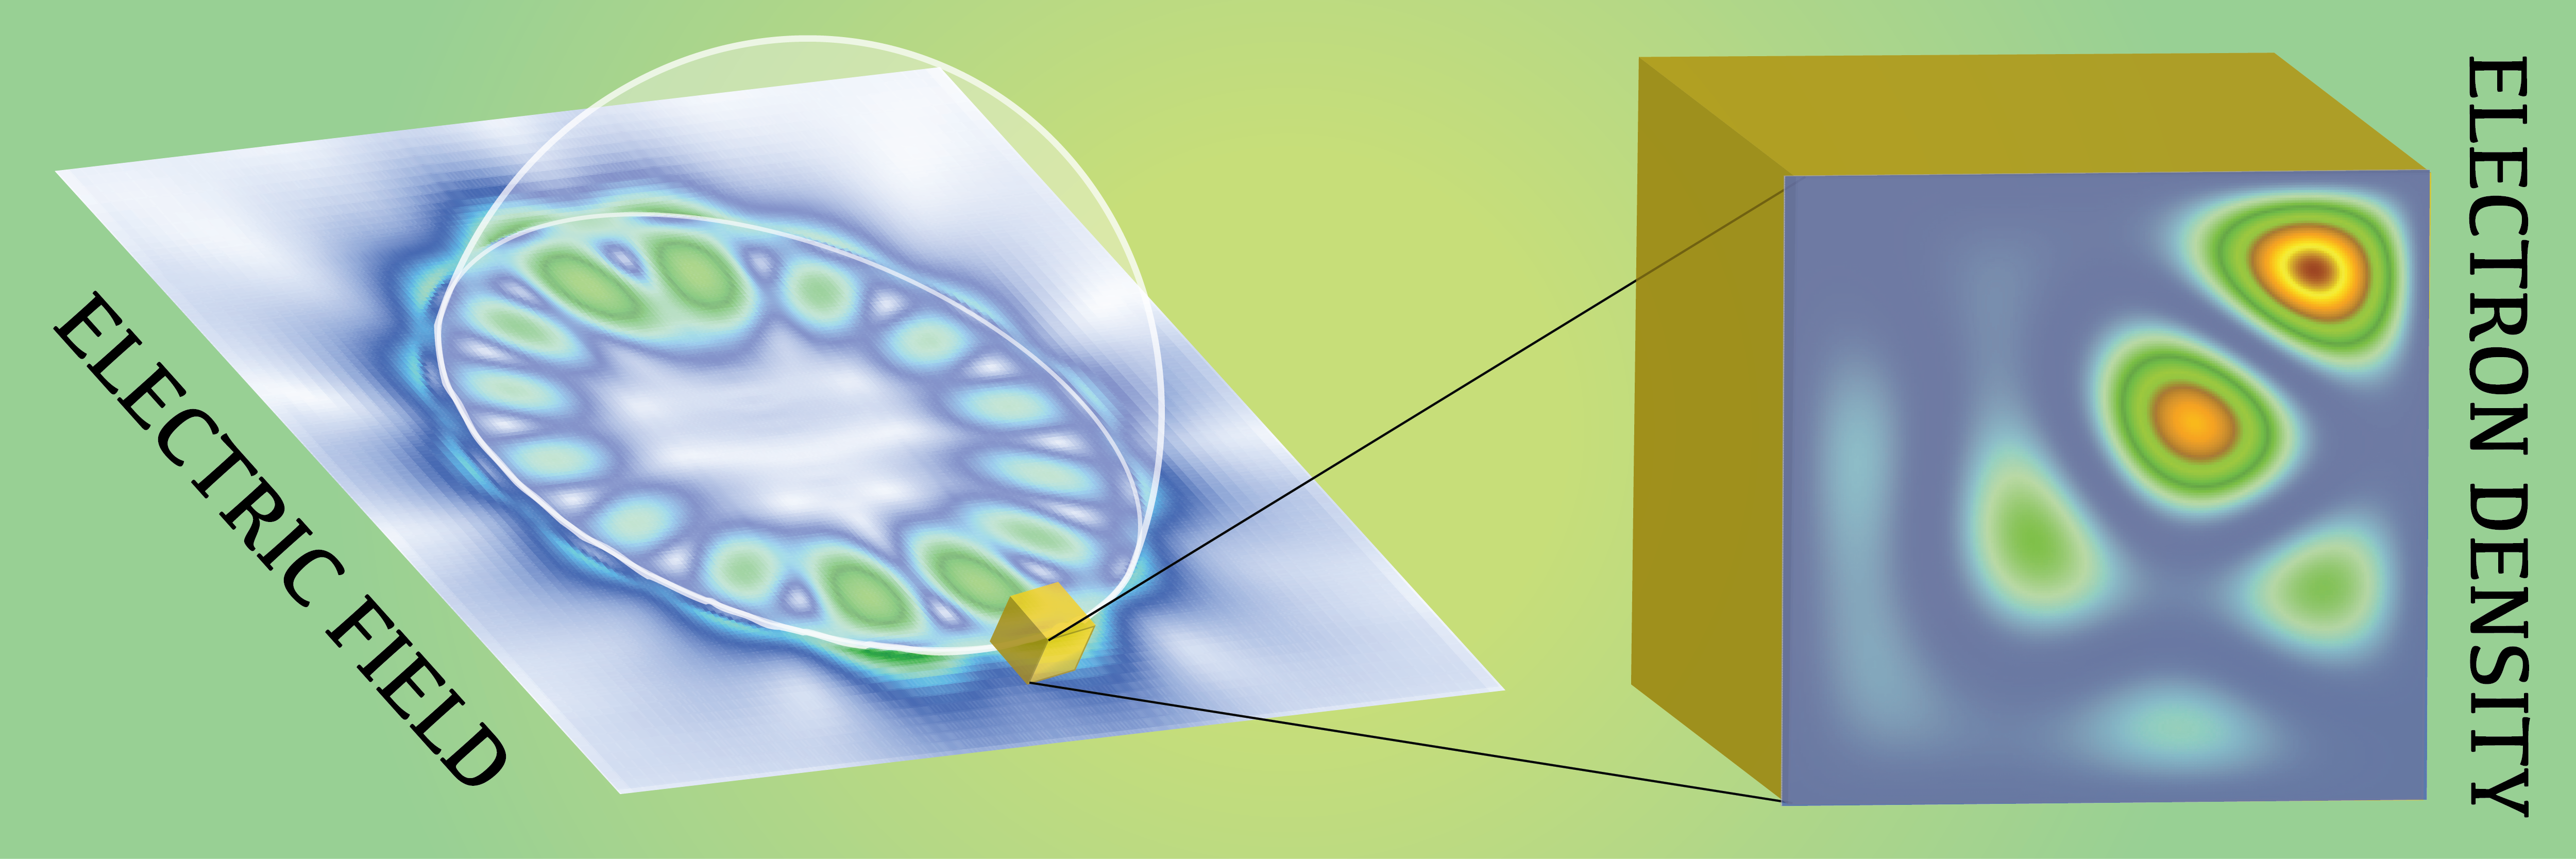
\includegraphics[width=9cm]{nanosphere_WGMv3.png}
\end{tocentry}

\begin{abstract}
What we present - interactive approach to studying the properties of real gasses.
Basis of this approach - a DIY molecular dynamics program that enables students to
interact with kinetic theory concepts in a variety of ways:
(a) visualization of trajectories under a variety of conditions, reinforcing
and clarifying fundamental concepts of particulate nature of matter and gas properties
(b) programming kinetic theory expressions that connect the microscopic quantities
    that are directly computed by MD simulations (velocity, change in momentum) to 
    macroscopic quantities T and P
(c) Novel opportunities to quantitatively and qualitiatively evaluate deviations from ideal gas behavior.  
A simple and fully-functional molecular dynamics code is provided written in simple C code that can be compiled
and run on Windows, Mac, and Linux platforms.

Excercises:
(1)  Compute R and Z for several scenarios, visualize trajectories, compare Z to VDW equation
(2)  Determine Boyl temperatures
(3)  Compare isotherms with VDW equation

%This manuscript presents an exercise that utilizes
%mathematical software to explore Fourier transforms in the context
%of model quantum mechanical systems, thus providing a deeper
%mathematical understanding of relevant information often introduced
%and treated as a “black-box” in analytical chemistry courses.
%The exercise is given to undergraduate students in their third year
%during physical chemistry, thus providing a theoretical foundation
%for the subsequent introduction of such material in analytical
%instrumentation courses. With the reinforcement of familiar
%concepts such as the Heisenberg Uncertainty Principle, classical correspondence, and linear combinations in the context of
%both position and momentum space for a particle in a box, a better understanding of the mathematical implications of the Fourier
%transform is fostered. Subsequent analysis of a time-dependent function constructed via a linear combination and its
%transformation to the frequency domain provides a practical example relating to the Fourier processes applied in analytical
%spectroscopy. The final portion of the exercise returns to the position/momentum conjugate pair and explores how the
%construction of a narrow wavepacket via a sum of cosines illustrates the Uncertainty Principle once the probability density
%functions of each coordinate are analyzed. This exercise has been shown to not only reinforce fundamental concepts necessary for
%a true appreciation of quantum mechanics, but also help demystify the Fourier transform process for students taking analytical
%chemistry.
%KEYWORDS: Upper-Division Undergr

\end{abstract}

%%\maketitle

%%\end{document}

\section{Introduction}
%%% Why are gasses important to chemistry
The study of gasses has enabled a tremendous number of insights into the nature of chemical 
structure and reactivity, %perhaps enumerate some examples here... molecular beams, old gas law experiments, others???
The study of gasses continues
to have substantial pedagogical relevance.  Gasses are introduced in the elementary science curriculum as one of the 
the fundamental states of matter, providing perhaps the first notion to students that matter is all around us all the time.   %%% Reference for this
Chemistry students encounter the ideal gas law throughout their education and in a variety of contexts.  
The ideal gas law is an important part of the particle theory of matter, and is useful in illustrating and quantifying
the relationships between different measurable quantities that characterize a gas system.  The ideal gas law is also 
used extensively to motivate thermodynamic processes and cycles, and the changes in energy and entropy associated with them.  
Gasses also provide arguably the simplest regime for analyzing intermolecular interactions.  The fact that the ideal gas law
has such remarkable predictive power in a variety of circumstances despite its neglect of intermolecular interactions illustrates
important concepts about the distance dependence of these forces.  That is, the average intermolecular distance is large in 
low-density gasses, therefore the average intermolecular force is negligible.  Despite repeated exposure,
undergraduate chemistry students struggle to develop both a functional understanding of the 
ideal gas law%\cite{}, 
and a solid conceptual understanding of the assumptions that define the ideal gas model (non-interacting point masses 
that undergo elastic collisions with the walls of their container).  We have observed in our own Physical Chemistry curriculum 
that students also struggle to develop a functional
understanding of ``real gas'' equations of state (e.g. Van der Waals equation) and sound
physical intuition about the microscopic intermolecular forces in gasses.  We conjecture that macroscopic equations of state,
microscopic models of intermolecular forces, and mental pictures of gaseous matter tend to lie in different conceptual domains, and
that this creates an impediment to a deep understanding of gas properties and behaviors across a vareity of chemically relevant contexts.

In this paper, we present a simulation module that can aid inquiry-driven study of gasses across
the continuum of regimes between ideal and non-ideal behavior.  The full commented source code of this simulation,
as well as directions for compiling and running the code on Windows, Mac, and Linux platforms, are distributed as a supplement
to this paper.  The simulation is based upon classical molecular dynamics
simulation of particles that interact through the Lennard-Jones potential.  In this technique, Newton's equations of motion 
are solved for all particles to render their motion in 3-dimensional space (i.e., molecular dynamics trajectories).  Our code outputs the coordinates
of each particle at each step in time in a format that can be readily rendered as an animation by the open-source program
VMD (instructions on obtaining and using VMD are also provided as a supplement).  Kinetic theory is used to
compute macroscopic quantities including the temperature, pressure, and compressibility (which is a measure
of deviation from ideality) from the time-average of the molecular dynamics trajectories.  Microscopic quantities like the kinetic
and potential energy of individual particles are also readily computed.  

In the remainder of the paper, we will provide an overview of the salient details of molecular dynamics simulations, including
a discussion of how macroscopic quantites are connected to the underlying microscopic information that molecular dynamics simulations directly provide.  We also provide 
several suggestions for how to leverage these simulations for inquiry-driven excercises that can enable students to discover
connections between microscopic and macroscopic properties of gasses, and also to develop a intuitive mental 
model of the behavior of gasses in ideal and non-ideal regimes.  We will conclude with suggestions for future advances
that can leverage molecular simulation to advance students comprehensive of properties and processes of gasses.  

\section{Overview of Molecular Dynamics Simulations}
Aneesur Rahman is credited as the pioneer of Molecular Dynamics (MD) simulations, having developed the first computer
program to simulate the motion of a system of 864 Argon atoms in 1964.%~\cite{Rahman}
The underlying concept behind MD simulations is remarkably simple:  atoms and molecules exert forces on one another that affect their motion,
and the changes in motion due to these forces can be predicted to high accuracy by solving classical equations of motion (i.e. Newton's Law).
This is concept is similar in spirit to the types of kinematics problems students encounter in first year physics: identify
the forces acting on a particle (e.g. a baseball), then find its position and velocity at some time in the future given its current
position and velocity along with its mass.  
The two challenges in the case of MD simulations are the calculation of the appropriate forces on the particles and the 
solution of the equations of
Newton's Law for the very large number $N$ of particles that arise in typical simulations.  A variety of computer algorithms are
available that permit Newton's Law to be solved for many thousands of atoms even with modest computational resources.
In this work, we utilize the velocity verlet algorithm to update the positions and velocities of
the particles once the forces have been computed.     
The velocity verlet algorithm updates the positions of each particles from time $t$ to time $t + dt$ according to 
\begin{equation}
\vec{r}_{i}(t+dt) = \vec{r}_{i}(t) + \vec{v}_i(t) \: dt + \frac{1}{2} \vec{a}_i(t) \: dt^2 
\end{equation}
where $\vec{r}_{i}(t)$ represents the position vector of the $i^{th}$ particle at time $t$, 
$\vec{v}_i(t)$ represents the velocity vector of the $i^{th}$ particle at time $t$, and
$\vec{a}_i(t)$ is the acceleration vector of the $i^{th}$ particle at time $t$.  In our MD program,
we use a coordinate system so $\vec{r}$  has an $x$, $y$, and $z$ component:  $\vec{r} = x \: \hat{i} + y \: \hat{j} + z \: \hat{k}$,
and similarly for $\vec{v}$ and $\vec{a}$.  The velocity is updated from time $t$ to time $t+dt$ according to
\begin{equation}
\vec{v}_i (t+1) = \vec{v}_i (t) +  \frac{1}{2} \vec{a}_i(t) \: dt.
\end{equation}

The typical approach to calculating the forces is first to specify a potential energy function for the particles
that models the change in potential energy due to the attractive interactions atoms and molecules experience
at moderate separations, and the repulsive interactions they experience at small separations.  The forces on the particles
are then calculated from the derivative of this function;
\begin{equation}
\vec{F}_i = \sum_{j \neq i}^N - \frac{d V( \vec{r}_{ij}) }{d \vec{r}_{ij}}.
\end{equation}
In the above expression, $\vec{F}_i$ is the total force experienced on the $i^{th}$ particle in a $N$ particle system
due to its interaction with all of the remaining $N-1$ particles, and $\vec{r}_{ij}$ is the separation between
particles $i$ and $j$, defined as $\vec{r}_{ij} = \vec{r}_i - \vec{r}_j$.  This expression assumes pair-wise interactions only contribute to the forces, this assumption
can be very poor in some systems (e.g. water), as has been discussed extensively (see, for example, ....).  
In Rahman's original work, and in the present work, an simple pair potential known as the Lennard-Jones potential 
is used,
\begin{equation}
V( \vec{r}_{ij}) = 4 \epsilon \left( \left( \frac{\sigma}{\vec{r}_{ij}} \right)^{12} - \left(\frac{\sigma}{\vec{r}_{ij}} \right)^6 \right),
\end{equation}
where the $\epsilon$ parameter defines the interaction strength and the $\sigma$ parameter defines the effective
lengthscale of the interactions, which could be analogized to concepts like the Van der Waals radius of the atom or molecule.
The specific value of these parameters can be obtained by experimental and theoretical methods.  Remarkably, Rahman's early
work simulating liquid Argon showed that this simple potential leads to the emergence of a large number of macroscopic properties 
that tracked experimental measurements with surprising fidelit. %\cite{Rahman}.
Importantly, the derivative of the L-J potential is smooth everywhere, which means the force is well defined
at all separations, 
\begin{equation}
\vec{F}_{ij}(\vec{r}_{ij}) = \frac{23 \epsilon}{\sigma^2} \vec{r}_{ij} \left( 2\left(\frac{\sigma}{r_{ij}}\right)^{14} - \left(\frac{\sigma}{r_{ij}}\right)^8\right)
\end{equation}

Pressure
\begin{equation}
P(t) = \sum_i^N = 2 m \vec{v}_i(t)
\end{equation}

Temperature
\begin{equation}
T(t) = \frac{ m \langle v^2 (t) \rangle }{3 k_B}
\end{equation}

MVS
\begin{equation}
\langle v^2 \rangle = \frac{1}{N} sum_i^N \vec{v}_i(t)
\end{equation}

The thermodynamic pressure and temperature can be determiend from the time average of
the instantaneous $T$ and $P$.  

Each simulation is defined
by an initial temperature, the number of particles being simulated, the volume in which the particles are enclosed,
and by microscopic details of the particles, including mass and the Lennard-Jones parameters.  The initial temperature
is used to define the distribution of initial velocities of the particles, while the volume and number of particles is used
to define the initial positions of the particles (see Supplemental Information for more details).  The version of the code
we provide has the Lennard-Jones parameters for Argon%\cite{MC_Reference_Ar}
hard-coded in, and we provide alternative Lennard-Jones parameters for other noble gasses in the supplemental information.
The

We believe this simulation module can be an important tool towards connecting conceptual domains of macroscopic gas behavior,
microscopic interaction pictures, and mental models of gasseous matter.

%%% What makes them hard to understane
Studies have suggested the difficulty students have developing a functional understanding of gas properties
arises from misconceptions students have about the microscopic behaviors of gasses.
Developing a sound intuition for the behavior of gassess in the continuum of regimes between ideal and non-ideal
behavior is challenging because we can't see them.
Computer simulation can help bridge this gap, allowing interactions at a variety of levels
- Underlying physical model of intermolecular forces (L-J)
- Kinematics resulting from that model (F=ma)
- Emergence of Pressure and Temperature from Kinematics
- Analysis of gas properties from emergent quantities
- Visualization of individual trajectories and collective behavior
- Numerical experimentation with various conditions and processes to extract and analyze properties of interest




\section{Associated Content}
Additional Figures illustrating hot carrier distributions and dynamics, as well as details of the time-dependent
configuration interaction singles method and the finite-difference time domain simulations are provided in the Supporting 
Information.  This material is available free of charge via the Internet at http://pubs.acs.org

\section{Author Information}
{\bf Corresponding Author}
$^*$ Email: foleyj10@wpunj.edu
\newline
$^{\dagger}$  C.S. and O.A. contributed equally to this work.
\newline
The authors declare no competing financial interest.

\section{Acknowledgment}
JJF Acknowledges the College of Science and Health for startup support.


\bibliography{MD} 

\end{document}
   

